% SAE Faithfulness paper. Build: cd research_paper/Latex && latexmk -pdf main.tex
% Tables in tables/ and figures in ../Latex_Fig/ are GENERATED by scripts/shared/build_paper_artifacts.py from
% committed result files; do not edit them by hand. Journal template: not chosen yet (Review #8 asks by 11-17);
% this neutral article class is meant to be ported.
\documentclass[11pt]{article}
\usepackage[margin=1in]{geometry}
\usepackage[T1]{fontenc}
\IfFileExists{lmodern.sty}{\usepackage{lmodern}}{}
\usepackage{amsmath,amssymb}
\usepackage{booktabs}
\usepackage{adjustbox}
\usepackage{graphicx}
\usepackage{xcolor}
\usepackage[numbers,sort&compress]{natbib}
\usepackage[hidelinks]{hyperref}
\graphicspath{{../Latex_Fig/}}

\newcommand{\pending}[1]{\noindent\fcolorbox{orange}{orange!8}{\parbox{\dimexpr\linewidth-2\fboxsep-2\fboxrule}{\small\textbf{PENDING:} #1}}\par\medskip}
\newcommand{\evlabel}[1]{\textsc{#1}}

\title{Do Sparse Autoencoders Preserve What a Language Model Uses?\\
\large A Layer-wise Audit of Reconstruction, Information, Behavioural and Causal Faithfulness in GPT-2 Small}
\author{Aditi Shukla \and Dhruv Rai \and Simbanegavi Simbarashe\\
\small DATS 6501 Data Science Capstone, The George Washington University}
\date{Draft of \today}

\begin{document}
\maketitle

\begin{abstract}
Sparse autoencoders (SAEs) are widely used to explain what large language models represent, which presumes that an
SAE is a faithful stand-in for the activations it replaces. We audit that presumption at all twelve layers of GPT-2
Small for three SAE architectures (ReLU, TopK and a sigmoid-surrogate JumpReLU; 108 SAEs at matched sparsity, three
seeds each), separating four levels of faithfulness: reconstruction, task-information preservation, behavioural
faithfulness and causal faithfulness. Reconstruction degrades with depth (OWT test explained variance 0.93--0.95 at
layers 0--2, 0.76--0.82 at layer 11). Within a layer, reconstruction error predicts how much splicing the SAE damages
the model's predictions, but not how much truth information is lost. The apparent collapse of a frozen truth probe
on SAE reconstructions is largely reproduced by random noise of the same norm; re-trained readers show a smaller but
real loss, and at equal reconstruction error the SAEs never preserve task information better than PCA. Using an
equal-length persona-instruction task built to remove a length shortcut, we locate where GPT-2 carries the
instruction's effect and decompose it: the SAE-reconstructed activation difference restores 93--97\,\% of the effect
at the layer-1 persona token but only 62--68\,\% at the layer-8 and layer-11 final token, with the remainder in the
reconstruction error or in an interaction between reconstruction and error. Short fine-tuning at layers 3, 6, 8 and 9
separates these levels again. Reconstruction fine-tuning on truth statements cuts their reconstruction error by
61--85\,\% and lowers the truth gap measured by a probe frozen on original activations, meeting its pre-registered
criterion in 4 of 9 layer--architecture cells beyond layer 6; re-trained probes, however, show no consistent gain,
so we do not claim that truth information is recovered. Adding an output-KL term improves behavioural faithfulness
in 5 of 9 creditable cells (in the other 4 the SAE's sparsity drifts beyond the pre-registered guard) and never
improves truth preservation. All results except the reconstruction table are \evlabel{validation} findings, not confirmed results;
a single pre-registered held-out evaluation is pending.
\end{abstract}

\pending{Abstract to be revised after E1--E3 and the final held-out evaluation (M5). Numbers above are validation-stage unless marked \evlabel{test}.}

\section{Introduction}\label{sec:intro}

Sparse autoencoders decompose a model's dense activations into a larger set of sparsely active latents, many of which
look human-interpretable \citep{bricken2023monosemanticity,cunningham2023sparse}. They have become a standard tool of
mechanistic interpretability, with architectures that trade off reconstruction against sparsity in different ways
\citep{gao2024scaling,rajamanoharan2024jumping}. Interpretability claims made through an SAE --- that the model
represents truth with certain features, or that a feature controls a behaviour --- inherit an assumption: that the
SAE is a \emph{faithful} replacement for the activation it reconstructs.

Faithfulness has several distinct meanings that are often conflated:
\begin{enumerate}
  \item \textbf{Reconstruction}: the reconstruction $\hat{x}$ is close to the activation $x$.
  \item \textbf{Information preservation}: task information that the model encodes (here, whether a statement is true;
        whether a persona instruction is honest) can still be read from $\hat{x}$.
  \item \textbf{Behavioural faithfulness}: the model behaves the same when $\hat{x}$ replaces $x$.
  \item \textbf{Causal faithfulness}: $\hat{x}$ carries the specific causal effect the model uses for a task.
\end{enumerate}
Explained variance is dominated by high-variance directions shared by all inputs, while task-relevant differences can
be small, low-variance directions. Good reconstruction therefore does not guarantee the other three properties. This
paper measures each level separately, at every layer of GPT-2 Small \citep{radford2019gpt2}.

\paragraph{Contributions.}
\begin{itemize}
  \item A matched-sparsity comparison of ReLU, TopK and JumpReLU SAEs at all 12 layers of GPT-2 Small, with three seeds
        (\S\ref{sec:recon}).
  \item A four-level information test that separates readout shift from information loss using frozen and re-trained
        readers, norm-matched noise and PCA references (\S\ref{sec:info}).
  \item A within-layer analysis showing that reconstruction error predicts behavioural damage but not truth readout,
        and that earlier pooled correlations were artefacts of mixing layers (\S\ref{sec:behaviour}).
  \item A shortcut-free persona-instruction task, a pre-registered causal site sweep, and a decomposition of the
        causal effect into reconstruction, error and interaction parts (\S\ref{sec:causal}).
  \item Pre-registered fine-tuning experiments, including an audit that found our own earlier truth-aware objective
        to be circular (\S\ref{sec:finetune}).
\end{itemize}

\paragraph{Scope of the claims.} All in-house SAEs have 3072 latents (4$\times$ expansion), target L0 = 128 and are
trained on 101{,}600 OpenWebText tokens. The results describe these SAEs; whether they hold for larger, longer-trained
SAEs is tested only partially (\S\ref{sec:limits}).

\pending{Final framing paragraph (Review \#8: lead with the audit's negative finding) after IMP-L and M5.}

\section{Related Work}\label{sec:related}

\paragraph{Sparse dictionary learning for interpretability.} \citet{bricken2023monosemanticity} and
\citet{cunningham2023sparse} showed that SAEs trained on transformer activations yield many interpretable latents.
\citet{gao2024scaling} introduced TopK SAEs and studied scaling; \citet{rajamanoharan2024jumping} introduced JumpReLU
SAEs with a learned threshold and a straight-through estimator. Our JumpReLU uses a simpler sigmoid surrogate and is
not the published estimator (\S\ref{sec:setup}). Public SAE suites exist for GPT-2 Small via SAELens
\citep{saelens2024} and for Gemma 2 via Gemma Scope \citep{gemmascope2024}.

\paragraph{Evaluating SAEs beyond reconstruction.} SAEBench \citep{karvonen2025saebench} evaluates SAEs on a broad set
of downstream metrics and finds that proxy metrics such as reconstruction and sparsity do not reliably predict
practical usefulness. AxBench \citep{wu2025axbench} finds that simple baselines outperform SAE-based methods for
concept detection and steering. \citet{paulo2024automatic} automate the interpretation of SAE features at scale. Our
audit is narrower but more controlled: one model, one task family per question, and pre-registered comparisons with
explicit noise, PCA and synonym controls.

\paragraph{Training for downstream faithfulness.} \citet{braun2024e2e} train SAEs end-to-end with a KL objective on the
model's output. Our output-KL fine-tuning (\S\ref{sec:finetune}) is inspired by this but is not a reproduction: it
fine-tunes existing local SAEs for 500 steps and keeps the local reconstruction term.

\paragraph{Truth and honesty representations.} \citet{marks2023geometry} find linear truth structure in LLM
activations (the Geometry of Truth datasets we use); \citet{zou2023representation} introduce representation
engineering with persona-contrast prompts, from which our original RepE task was derived.

\pending{Expand to the 15-reference review from PR \#16 (Review \#8 H3b); add a differentiation statement per work.
Every citation must be checked against the original paper before submission.}

\section{Background: Transformer Activations and SAEs}\label{sec:background}

GPT-2 Small has 12 transformer blocks with a residual stream of width $d=768$. We study the activation entering block
$L$, \texttt{blocks.$L$.hook\_resid\_pre}, for $L=0,\dots,11$; at $L=0$ this is the token plus position embedding.

An SAE with $m$ latents maps $x\in\mathbb{R}^d$ to
\begin{equation}
  z=\sigma\big(W_e(x-b_d)+b_e\big)\in\mathbb{R}^m,\qquad \hat{x}=W_d z+b_d,\qquad e=x-\hat{x},
\end{equation}
with decoder columns renormalised to unit norm after every optimisation step. The three activation functions are
\begin{align}
  \text{ReLU:}\quad & z=\mathrm{ReLU}(p), && \text{penalty } \textstyle\sum_i z_i,\\
  \text{TopK:}\quad & z=\mathrm{TopK}_k\big(\mathrm{ReLU}(p)\big),\ k=128, && \text{no penalty},\\
  \text{JumpReLU (surrogate):}\quad & z=\mathrm{ReLU}(p)\odot H(p-\theta), && \text{penalty } \textstyle\sum_i \sigma\big((p_i-\theta_i)/T\big),
\end{align}
where $p$ is the pre-activation, $H$ the step function and $\theta$ a learned per-latent threshold whose gradient uses
a sigmoid straight-through estimator with $T=0.1$. The training loss is $\mathrm{MSE}(\hat{x},x)+c\cdot\text{penalty}$,
and a multiplicative controller adjusts $c$ every 25 steps towards a target L0 of 128.

\paragraph{Metrics.} Explained variance is $\mathrm{EV}=1-\sum\|x-\hat{x}\|^2/\sum\|x-\bar{x}\|^2$ and
$\mathrm{NMSE}=1-\mathrm{EV}$; L0 is the mean number of active latents. An AUROC gap is
$\mathrm{AUROC}(x)-\mathrm{AUROC}(\hat{x})$ for a given reader. Spliced $\Delta$CE is the increase in next-token
cross-entropy when $\hat{x}$ replaces $x$ at every non-BOS position; loss recovered is
$(\mathrm{CE}_{\text{mean-abl}}-\mathrm{CE}_{\text{SAE}})/(\mathrm{CE}_{\text{mean-abl}}-\mathrm{CE}_{\text{orig}})$.
Causal quantities are defined in \S\ref{sec:causal}.

\section{Research Questions and Hypotheses}\label{sec:questions}

\textbf{Main question.} Can SAE reconstruction of frozen LLM activations be improved while preserving truth-related
information and causal behaviour across transformer layers?

\begin{description}
  \item[SQ1 (reconstruction).] How do ReLU, TopK and JumpReLU SAEs compare across the 12 layers at matched sparsity?
  \item[SQ2 (information).] Which task information survives reconstruction, and is the loss specific to SAEs compared
        with generic perturbations of the same size and with PCA at the same reconstruction error?
  \item[SQ3 (behaviour).] How much does splicing the SAE in damage GPT-2's predictions, and does reconstruction error
        predict that damage between SAEs at the same layer?
  \item[SQ4 (causal).] Where does GPT-2 carry a persona-instruction effect, and how much of it survives in the SAE
        reconstruction?
  \item[SQ5 (improvement).] Can fine-tuning improve faithfulness at matched sparsity, and at which layers?
\end{description}

\paragraph{Evidential status.} Each result is labelled \evlabel{test} (held-out split, evaluated once under a written
protocol), \evlabel{validation}, or \evlabel{preliminary} (a validation pilot whose pre-registered criterion was not met
or which is unreplicated). Every experiment from M0 onwards was pre-registered with file hashes before it ran.

The project's original proposal asked whether SAE features are causally faithful to their auto-generated labels. The
scope was narrowed to the questions above after instructor reviews and internal audits (Appendix~\ref{app:history}).

\section{Datasets and Experimental Setup}\label{sec:setup}

\paragraph{OpenWebText (OWT).} 1000 documents sampled from \texttt{Skylion007/openwebtext} (streaming shuffle, seed
42, 100--20{,}000 characters, exact deduplication), split 800/100/100 by document. Each document is truncated to 128
tokens; excluding BOS this gives 101{,}600 / 12{,}700 / 12{,}700 training, validation and test tokens.

\paragraph{Geometry of Truth (GoT).} The \texttt{cities} and \texttt{neg\_cities} sets \citep{marks2023geometry}
(1496 statements each) form the ``geographic'' truth task, with city-grouped splits of 1046/224/226 per set. The
numerical sets have a surface shortcut (the second number alone gives AUROC 0.84) and are used only as a diagnostic.

\paragraph{RepE-LM persona task.} Our original persona prompts (``Pretend you're an honest/untruthful person'') had a
length shortcut: \emph{untruthful} is three tokens longer than \emph{honest}, and prompt length alone predicts the
label with AUROC 0.80. We therefore built RepE-LM: 506 statements (train 417, validation 89) times 20 prompt variants,
in which the two prompts of each pair differ in exactly one token at a fixed position. Templates T1--T4 swap
truthful/deceptive, trustworthy/dishonest, sincere/lying and facts/lies, each with an honest-synonym control; T5--T6
are held out; N1--N2 swap neutral words (tall/short, red/blue). Seven pre-registered gates (Table~\ref{tab:m1})
verify the construction.

\paragraph{SAE training.} For each layer, architecture and seed (42, 1042, 2042) we train one SAE with width 3072,
Adam (learning rate $3\times10^{-4}$), batch 256 sampled with replacement, gradient clipping at 10, and one
uninterrupted run of 15{,}000 steps (3.84M samples, about 38 passes over the training tokens). Architectures are
compared only when every run's L0 is within $\pm$10\,\% of the target; 107 of 108 runs qualify (layer-0 JumpReLU seed
42 does not).

\paragraph{Splits.} Probes and selections use training data; results are reported on validation unless labelled
\evlabel{test}. The RepE-LM test split has never been built or accessed. The GoT test split was scored in earlier
frozen-probe evaluations and is treated as previously exposed (Appendix~\ref{app:exposure}).

\paragraph{Evidence status of every result in this paper.} Apart from the OWT reconstruction table
(\evlabel{test}), \emph{every} result reported here (M0--M4 and the fine-tuning experiments) is a
\evlabel{validation} finding. Hypotheses, criteria and scripts were fixed before each run, but the held-out test
evaluation (M5) has not been run, so no result is a confirmed held-out finding. When a site or effect selected on training prompts
is said to have \emph{replicated}, it means only that it held again on validation prompts. Fine-tuning
classes (\evlabel{preliminary improvement}, \evlabel{no improvement}, \evlabel{not creditable},
\evlabel{regression}) are validation classes; none of them is a confirmed result.

% generated by scripts/shared/build_paper_artifacts.py from results/repe/repe_lm_gates/gates.json
\begin{table}[t]
\centering
\small
\caption{M1 RepE-LM construction and gates (pre-registered pass rules). Source: \texttt{results/\allowbreak{}repe/\allowbreak{}repe\_lm\_gates/\allowbreak{}gates.json}.}
\label{tab:m1}
\begin{adjustbox}{max width=\linewidth}
\begin{tabular}{llp{0.62\linewidth}}
\toprule
Gate & Status & Evidence (train statements) \\
\midrule
K1 construction & PASS & 6,072 pairs; max residual difference before the swapped token 0.0 at all 12 layers \\
K2 shortcuts & PASS & max deviation of any shortcut AUROC from 0.5: 5.6e-17 \\
K3 positive control & PASS & unmasked bag-of-words AUROC 1.000 \\
K5 persona meaning & PASS & leave-one-pair-out AUROC 0.701 at layer 8 (CI low 0.689); passing layers [8, 11] \\
K6 leakage & PASS & 0 exact overlaps; 0 same-label near-duplicates \\
K7 behaviour & PASS & median KL(H$\|$U) 0.0186 vs KL(H$\|$H$^\prime$) 0.0092 nats; ratio 1.99; Wilcoxon $p=3e-68$ \\
\bottomrule
\end{tabular}
\end{adjustbox}
\end{table}


\section{Reconstruction and Sparsity}\label{sec:recon}

Table~\ref{tab:recon} and Figure~\ref{fig:recon} (left) give OWT test reconstruction for all 108 SAEs
(\evlabel{test}). Explained variance falls with depth for every architecture, from 0.93--0.95 at layers 0--2 to
0.757 (ReLU) and 0.815 (TopK, JumpReLU) at layer 11. Among matched runs, ReLU leads at layer 1, ReLU and JumpReLU tie
at layer 2, JumpReLU leads at layers 3--9, and JumpReLU and TopK tie at layers 10--11. Seed standard deviations are
$\le 0.001$ except for layer-0 JumpReLU, whose seed 42 is unmatched (L0 73.6; about 96\,\% of latents dead) and
excluded from rankings.

\paragraph{Sparsity is matched on OWT only.} ReLU runs 2--6\,\% above the target L0. A within-layer adjustment using
the L0 elasticity measured in an earlier sweep changes no ranking except two near-ties (M0). The architectures differ
strongly in effective width: of 3072 latents, ReLU keeps 2920--3063 alive, TopK 1711--2851 and JumpReLU 469--2947. On
task prompts the number of active latents is not matched (on GoT final tokens, TopK uses 128, ReLU 32--110 and
JumpReLU 23--92 at layers 1--11), which confounds architecture comparisons on task information (\S\ref{sec:info}).

% generated by scripts/shared/build_paper_artifacts.py from results/openwebtext/reconstruction_evaluation/uninterrupted_protocol/all_layers_summary.csv
\begin{table}[t]
\centering
\small
\caption{Reconstruction on the OWT test split (TEST; 12{,}700 tokens), width 3072, target L0 = 128. Layer-0 JumpReLU includes the unmatched seed 42 (L0 73.6). Source: \texttt{results/\allowbreak{}openwebtext/\allowbreak{}reconstruction\_evaluation/\allowbreak{}uninterrupted\_protocol/\allowbreak{}all\_layers\_summary.csv}.}
\label{tab:recon}
\begin{adjustbox}{max width=\linewidth}
\begin{tabular}{rcccccc}
\toprule
Layer & \multicolumn{3}{c}{OWT test EV (mean$\pm$sd, 3 seeds)} & \multicolumn{3}{c}{OWT test L0} \\
\cmidrule(lr){2-4}\cmidrule(lr){5-7}
 & ReLU & TopK & JumpReLU & ReLU & TopK & JumpReLU \\
\midrule
0 & 0.950$\pm$0.000 & 0.911$\pm$0.000 & 0.826$\pm$0.101 & 135.1 & 125.3 & 110.3 \\
1 & 0.937$\pm$0.000 & 0.921$\pm$0.001 & 0.933$\pm$0.000 & 132.2 & 128.0 & 129.3 \\
2 & 0.936$\pm$0.000 & 0.926$\pm$0.000 & 0.935$\pm$0.002 & 131.9 & 128.0 & 129.0 \\
3 & 0.905$\pm$0.000 & 0.906$\pm$0.000 & 0.915$\pm$0.001 & 131.7 & 128.0 & 129.1 \\
4 & 0.872$\pm$0.000 & 0.884$\pm$0.000 & 0.893$\pm$0.001 & 131.1 & 128.0 & 129.1 \\
5 & 0.848$\pm$0.000 & 0.868$\pm$0.000 & 0.875$\pm$0.000 & 130.8 & 128.0 & 129.0 \\
6 & 0.832$\pm$0.001 & 0.857$\pm$0.000 & 0.865$\pm$0.000 & 131.0 & 128.0 & 129.1 \\
7 & 0.819$\pm$0.001 & 0.850$\pm$0.000 & 0.855$\pm$0.000 & 131.4 & 128.0 & 129.9 \\
8 & 0.805$\pm$0.000 & 0.840$\pm$0.000 & 0.844$\pm$0.000 & 131.9 & 128.0 & 130.3 \\
9 & 0.789$\pm$0.001 & 0.831$\pm$0.000 & 0.833$\pm$0.000 & 132.4 & 128.0 & 131.0 \\
10 & 0.773$\pm$0.000 & 0.822$\pm$0.000 & 0.823$\pm$0.000 & 132.7 & 128.0 & 131.6 \\
11 & 0.757$\pm$0.001 & 0.815$\pm$0.000 & 0.815$\pm$0.000 & 133.2 & 128.0 & 132.1 \\
\bottomrule
\end{tabular}
\end{adjustbox}
\end{table}


\begin{figure}[t]
  \centering
  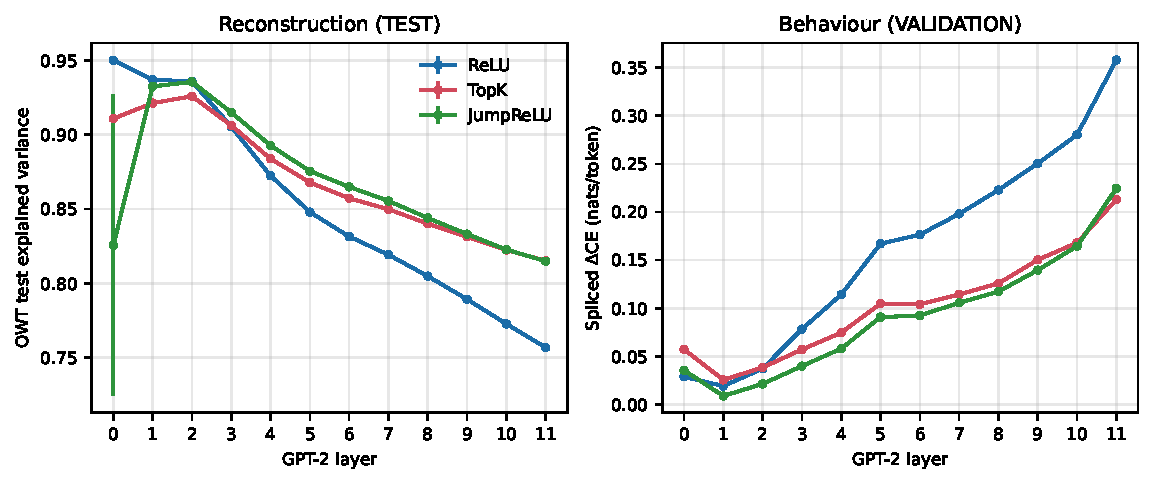
\includegraphics[width=\linewidth]{fig_reconstruction_behaviour}
  \caption{Left: OWT test explained variance by layer (\evlabel{test}; error bars: seed sd). Right: spliced
  next-token cross-entropy increase (\evlabel{validation}). Sources: Tables~\ref{tab:recon} and~\ref{tab:splice}.}
  \label{fig:recon}
\end{figure}

\pending{E1 (TopK trained at several $k$ to match task-level L0) and E2 (public \texttt{gpt2-small-res-jb}
reference; not matched in width, data or L0).}

\section{Information Preservation}\label{sec:info}

\paragraph{Frozen probes overstate the loss.} A logistic truth probe fitted on original activations and applied
unchanged to SAE reconstructions loses 0.28--0.29 AUROC on GoT (Table~\ref{tab:m2}, Figure~\ref{fig:m2}). Earlier
versions of this project read this as truth information being lost. Adding isotropic noise with the same norm as the
SAE error causes almost the same drop (0.25--0.26), and a simpler mass-mean reader loses only 0.02--0.03. Most of the
frozen-probe collapse is therefore sensitivity of that reader to any perturbation of this size, not SAE-specific loss.

\paragraph{A smaller, real loss remains.} Readers re-trained on the reconstructions are 0.07--0.12 AUROC worse than
readers trained on the original activations for GoT, and 0.14--0.18 worse for the persona task. Re-training never
recovers the original performance, so no cell is classified as ``readout shifted''; no cell is ``preserved''. The
task label can be decoded from the reconstruction error alone (AUROC 0.62--0.77), so the lost information is still in
the activation, outside the SAE's reconstruction.

\paragraph{SAEs are never better than PCA.} At the same OWT reconstruction error, PCA keeps at least as much task
information as the SAE in every cell; the SAE is significantly worse in 52 of 81 GoT cells, 59 of 99 persona cells
and 81 of 90 neutral cells (one-sided paired bootstrap, BH-corrected).

\paragraph{Persona versus generic change.} Part of the persona loss is generic one-word-change information: the
re-trained gap is 0.07--0.13 larger for persona than for neutral swaps at layers 3--8, and about equal at layers 10--11.

\paragraph{Architecture differences are confounded.} On truth, ReLU loses least and JumpReLU most, the reverse of
the reconstruction ranking; on persona, ReLU loses most. Because task-level L0 is not matched, we do not interpret
these differences as architecture effects until E1 is run.

% generated by scripts/shared/build_paper_artifacts.py from results/shared/m2_four_level_faithfulness/summary_by_layer_arch.csv
\begin{table}[t]
\centering
\small
\caption{M2 information preservation (VALIDATION): AUROC gaps (original $-$ reconstructed; $\downarrow$), mean over informative layers (GoT 4--11, RepE-LM 1--11) and 3 seeds. ``Noise adds isotropic noise with the norm of the SAE error; ``PCA is matched to the SAE's OWT validation NMSE. Error AUROC: label decoded from the error term alone. Source: \texttt{results/shared/m2\_four\_level\_faithfulness/summary\_by\_layer\_arch.csv}.}
\label{tab:m2}
\begin{adjustbox}{max width=\linewidth}
\begin{tabular}{llccccccc}
\toprule
Task & SAE & Frozen log. & Noise & Frozen m.-mean & Re-trained log. & PCA re-tr. & MLP & Error AUROC \\
\midrule
GoT & ReLU & 0.287 & 0.259 & 0.033 & 0.066 & 0.042 & 0.049 & 0.675 \\
GoT & TopK & 0.275 & 0.246 & 0.024 & 0.075 & 0.032 & 0.037 & 0.615 \\
GoT & JumpReLU & 0.286 & 0.257 & 0.026 & 0.118 & 0.030 & 0.066 & 0.632 \\
\midrule
Persona & ReLU & 0.198 & 0.076 & 0.091 & 0.179 & 0.131 & 0.232 & 0.773 \\
Persona & TopK & 0.162 & 0.072 & 0.066 & 0.147 & 0.116 & 0.190 & 0.719 \\
Persona & JumpReLU & 0.155 & 0.064 & 0.062 & 0.143 & 0.114 & 0.177 & 0.721 \\
\midrule
Neutral & ReLU & 0.113 & 0.048 & 0.049 & 0.099 & 0.066 & 0.033 & 0.636 \\
Neutral & TopK & 0.098 & 0.046 & 0.038 & 0.090 & 0.064 & 0.031 & 0.615 \\
Neutral & JumpReLU & 0.094 & 0.043 & 0.035 & 0.083 & 0.062 & 0.031 & 0.619 \\
\bottomrule
\end{tabular}
\end{adjustbox}
\end{table}


\begin{figure}[t]
  \centering
  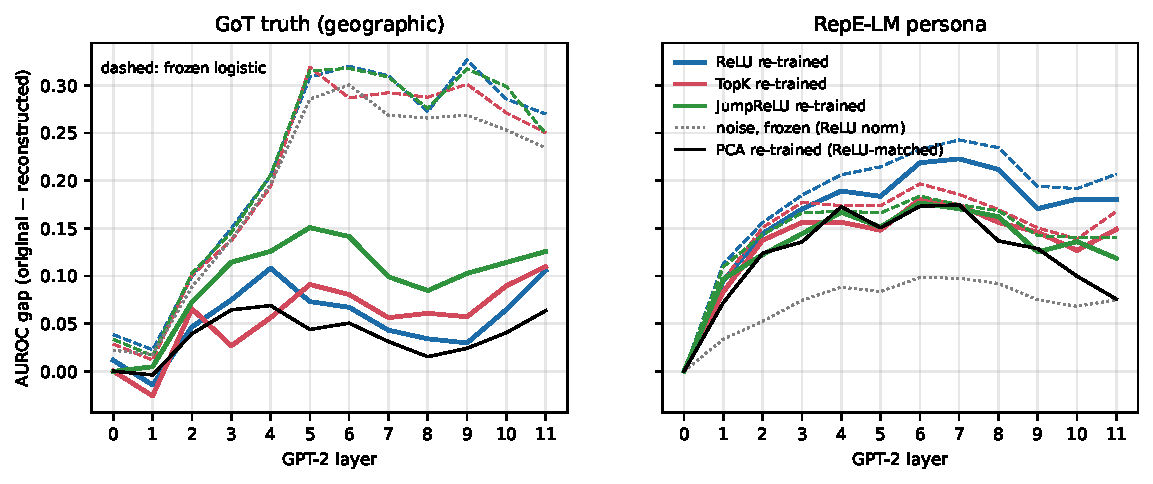
\includegraphics[width=\linewidth]{fig_m2_information}
  \caption{Information preservation by layer (\evlabel{validation}). Dashed: frozen logistic gap; solid: re-trained
  logistic gap; dotted grey: frozen gap under norm-matched noise; black: PCA at the ReLU SAE's error.}
  \label{fig:m2}
\end{figure}

\pending{M5 held-out confirmation; E1 task-level sparsity control; E2 external SAE reference.}

\section{Behavioural Faithfulness}\label{sec:behaviour}

Splicing the reconstruction into GPT-2 at every non-BOS position increases next-token cross-entropy by 0.009--0.026
nats at layer 1 and by 0.213--0.358 nats at layer 11 (Table~\ref{tab:splice}, \evlabel{validation}); loss recovered
relative to mean ablation stays at or above 0.93. An identity splice changes nothing (exactly 0). The true-versus-false
likelihood preference on GoT \texttt{cities} (0.82 originally) is unchanged within $\pm$0.025 through layer 8 and drops
by 0.04--0.09 at layers 9--11.

\paragraph{SAE error is more harmful than random error.} Replacing the SAE error by isotropic noise of the same norm
gives a smaller cross-entropy increase in most runs: the ratio of SAE-induced to noise-induced damage is 0.76--2.89
per run (median 1.64); 7 of 107 runs are below 1, all at layers 1--3.

\paragraph{Within a layer, reconstruction error predicts behavioural damage but not truth readout (M0).}
Table~\ref{tab:m0} reports within-layer regressions over the 107 matched SAEs. Lower OWT NMSE goes with less splice
damage ($\beta=0.165$ per unit log NMSE, Holm $p=0.0008$; per-layer Spearman $\rho$ 0.80--0.97 from layer 3). For the
frozen GoT truth gap, the formal test passes (Holm $p=0.044$), but architecture explains 99.8\,\% of the within-layer
NMSE variance and the association disappears without architecture fixed effects ($p=0.89$); GoT reconstruction error
has no association. Two earlier claims are corrected: a pooled correlation of 0.89 between reconstruction and persona
preservation is 0.05 within layer, and the range of the SAE-versus-noise damage ratio is the one given above.

% generated by scripts/shared/build_paper_artifacts.py from results/openwebtext/spliced_evaluation/summary.csv
\begin{table}[t]
\centering
\small
\caption{Behavioural faithfulness: GPT-2 with the SAE reconstruction spliced in at every non-BOS position (OWT validation; original CE 3.396 nats/token; matched seeds only). Source: \texttt{results/\allowbreak{}openwebtext/\allowbreak{}spliced\_evaluation/\allowbreak{}summary.csv}.}
\label{tab:splice}
\begin{adjustbox}{max width=\linewidth}
\begin{tabular}{rcccccc}
\toprule
Layer & \multicolumn{3}{c}{Spliced $\Delta$CE (nats/token, $\downarrow$)} & \multicolumn{3}{c}{Loss recovered ($\uparrow$)} \\
\cmidrule(lr){2-4}\cmidrule(lr){5-7}
 & ReLU & TopK & JumpReLU & ReLU & TopK & JumpReLU \\
\midrule
0 & 0.029 & 0.057 & 0.036 & 0.996 & 0.991 & 0.995 \\
1 & 0.019 & 0.026 & 0.009 & 0.998 & 0.997 & 0.999 \\
2 & 0.037 & 0.038 & 0.021 & 0.995 & 0.994 & 0.997 \\
3 & 0.078 & 0.057 & 0.040 & 0.987 & 0.991 & 0.994 \\
4 & 0.114 & 0.075 & 0.058 & 0.984 & 0.990 & 0.992 \\
5 & 0.167 & 0.105 & 0.091 & 0.967 & 0.980 & 0.982 \\
6 & 0.177 & 0.104 & 0.092 & 0.966 & 0.980 & 0.982 \\
7 & 0.198 & 0.114 & 0.106 & 0.963 & 0.979 & 0.980 \\
8 & 0.223 & 0.126 & 0.117 & 0.958 & 0.976 & 0.978 \\
9 & 0.250 & 0.150 & 0.140 & 0.951 & 0.971 & 0.973 \\
10 & 0.280 & 0.168 & 0.164 & 0.947 & 0.968 & 0.969 \\
11 & 0.358 & 0.213 & 0.225 & 0.930 & 0.958 & 0.956 \\
\bottomrule
\end{tabular}
\end{adjustbox}
\end{table}

% generated by scripts/shared/build_paper_artifacts.py from results/shared/m0_within_layer_reanalysis/within_layer_regressions.csv
\begin{table}[t]
\centering
\small
\caption{M0 within-layer regressions (VALIDATION): outcome $\sim\beta\cdot$predictor + layer FE + architecture FE + log L0, Freedman--Lane permutation within layer. The GoT row passes formally but vanishes without architecture fixed effects ($p=0.89$; see text). Source: \texttt{results/shared/m0\_within\_layer\_reanalysis/within\_layer\_regressions.csv}.}
\label{tab:m0}
\begin{adjustbox}{max width=\linewidth}
\begin{tabular}{lccccc}
\toprule
Predictor $\rightarrow$ outcome & $\beta$ & 95\% CI & $p_{\text{perm}}$ & $p_{\text{Holm}}$ & $n$ \\
\midrule
log OWT NMSE $\rightarrow$ GoT frozen-logistic gap & 0.268 & [0.056, 0.477] & 0.0146 & 0.0438 & 72 \\
log GoT relative error $\rightarrow$ GoT frozen-logistic gap & 0.005 & [-0.059, 0.080] & 0.8680 & 1.0000 & 72 \\
log OWT NMSE $\rightarrow$ OWT spliced $\Delta$CE & 0.165 & [0.134, 0.265] & 0.0002 & 0.0008 & 107 \\
log GoT relative error $\rightarrow$ OWT spliced $\Delta$CE & -0.012 & [-0.060, 0.028] & 0.6267 & 1.0000 & 107 \\
\bottomrule
\end{tabular}
\end{adjustbox}
\end{table}


\section{Causal Faithfulness}\label{sec:causal}

All results in this section are \evlabel{validation} findings (M3 sites selected on training prompts and
replicated on validation prompts; M4 on validation prompts).

\paragraph{Where GPT-2 carries the persona effect (M3).} For each RepE-LM pair we run GPT-2 on the honest (H) and the
dishonest (U) prompt and measure $\mathrm{KL}(p_H\|p_U)$ on the next token (mean 0.033 nats). Copying the honest
activation into the dishonest run at one layer and position group restores a share $E$ of that divergence.
Figure~\ref{fig:m3} shows that the effect is carried by the persona word early (layer 1: $E=0.97$) and by the final
token late (layer 11: $E=0.95$), with the handover at layers 7--8; the instruction words after the persona slot carry
up to 0.28. Of 65 cells, 50 pass the pre-registered test (Holm-corrected, above the 95th percentile of 200 matched-norm
random vectors). The pre-registered rule selected the layer-1 persona slot and the layer-11 final token, both
replicated on validation prompts; a pre-registered amendment added the layer-8 final token (train $E=0.505$), replicated
on validation without SAEs. A same-meaning synonym swap travels the same route at about half the size. Template T1 (truthful/deceptive) has
no effect beyond its synonym control and serves as a control case; T2--T4 are the primary set.

\begin{figure}[t]
  \centering
  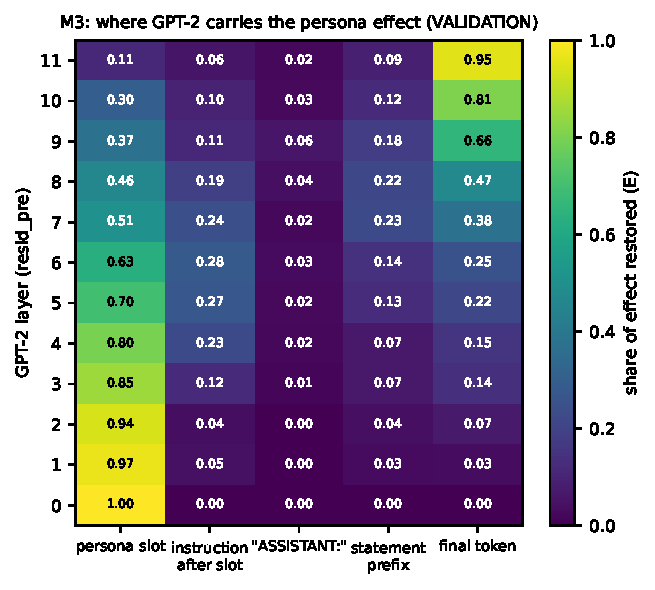
\includegraphics[width=0.62\linewidth]{fig_m3_sites}
  \caption{M3 (\evlabel{validation}): share of the persona-instruction effect restored by patching one position
  group at one layer of GPT-2 Small.}
  \label{fig:m3}
\end{figure}

\paragraph{How much of the effect the SAE carries (M4).} At a site, let $\Delta=x_H-x_U$, $\Delta_{\text{rec}}=\hat{x}_H-\hat{x}_U$
and $\Delta_{\text{err}}=e_H-e_U$, so $\Delta=\Delta_{\text{rec}}+\Delta_{\text{err}}$ exactly. With
$T(v)=\mathrm{KL}(p_H\|p_U)-\mathrm{KL}(p_H\|p_{U+v})$, we define $T_{\text{full}}=T(\Delta)$,
$T_{\text{rec}}=T(\Delta_{\text{rec}})$, $T_{\text{err}}=T(\Delta_{\text{err}})$, the interaction
$I=T_{\text{full}}-T_{\text{rec}}-T_{\text{err}}$, and Shapley shares $\phi_{\text{rec}}=(T_{\text{rec}}+T_{\text{full}}-T_{\text{err}})/2$.
The patch adds $v$ to the dishonest run's original activation; it is not a full splice. All exact checks pass
($\Delta$ identity error $9.5\times10^{-7}$; $T_{\text{full}}$ reproduces M3 to $7\times10^{-8}$).

Table~\ref{tab:m4} and Figure~\ref{fig:m4} show that the reconstructed difference restores 93--97\,\% of the effect at
the layer-1 persona token, but only 62--68\,\% at the layer-8 and layer-11 final token. There, ReLU's error part alone
carries 40--45\,\%; for TopK and JumpReLU, the interaction is large ($|I|/T_{\text{full}}$ 0.26--0.38), so their
shares cannot be read additively. The persona-minus-synonym difference is preserved in the reconstruction at every
site. Higher explained variance does not imply higher causal preservation: at layer 11, TopK has higher EV than ReLU
(0.815 vs 0.757) but keeps less of the effect (0.62 vs 0.68).

\paragraph{SAE-selected feature patches (error term kept).} Encoding both prompts, setting the dishonest prompt's top-$k$ features to
their honest values, decoding and keeping the error term restores more than 200 frequency- and magnitude-matched
random feature sets in all 27 SAE $\times$ site combinations ($p=0.005$, the minimum attainable). The effect is
distributed: one feature carries 2--10\,\% of $T_{\text{rec}}$ and 64 features 47--74\,\%. This shows that
SAE-defined directions are causally sufficient when inserted; it does not show that GPT-2 uses SAE features.

\paragraph{What these patches are, mathematically.} Because the error term is kept, every M4 patch has the form
$x_U+v$ with $v=W_{\text{dec}}(z'-z_U)$; the decoder bias cancels. $T_{\text{rec}}$ adds $v=W_{\text{dec}}(z_H-z_U)$
and the top-$k$ patch adds $W_{\text{dec},S}(z_{H,S}-z_{U,S})$. Each is therefore identical to adding one vector to
the dishonest prompt's raw activation. The same holds for any encode--edit--decode intervention that keeps the error,
including input-dependent clamps: $x'=x+W_{\text{dec}}(z'(x)-z(x))$. Because a dictionary of 3,072 or 12,288
latents spans $\mathbb{R}^{768}$, lying in decoder space does not restrict $v$. The only SAE-specific ingredient is how
$v$ is chosen: the encoder's input-dependent latent selection on the two prompts. The matched random-feature-set and
isotropic controls test that choice. The patches therefore establish that the SAE \emph{selects} input-dependent
directions that carry the effect when inserted. They do not establish an effect that is \emph{mediated} by the SAE,
which is what Review~\#8 asked of an SAE-in-the-loop intervention. Establishing mediation needs the downstream
computation to pass through SAE nonlinearities. Examples are an edit at layer $\ell$ with SAEs spliced at later
layers, or a run on $\hat{x}$ with no error term, compared against the spliced baseline. The layer-6 clamp
experiment (R2-clamp; input-dependent clamps, with and without the error term) found no supported effect
(\evlabel{validation}).

% generated by scripts/shared/build_paper_artifacts.py from results/repe/sae_patch_decomposition/architecture_summary.csv
\begin{table}[t]
\centering
\small
\caption{M4 causal decomposition (VALIDATION; templates T2--T4; mean$\pm$sd over 3 seeds). Shapley shares in parentheses are not interpretable as additive (pre-registered rule: interaction too large). Source: \texttt{results/\allowbreak{}repe/\allowbreak{}sae\_patch\_decomposition/\allowbreak{}architecture\_summary.csv}.}
\label{tab:m4}
\begin{adjustbox}{max width=\linewidth}
\begin{tabular}{llccccc}
\toprule
Site & SAE & $T_{\text{full}}$ (nats) & $T_{\text{rec}}/T_{\text{full}}$ & $T_{\text{err}}/T_{\text{full}}$ & $|I|/T_{\text{full}}$ & $\phi_{\text{rec}}$ \\
\midrule
L1 persona slot & ReLU & 0.0435 & 0.938$\pm$0.019 & 0.14 & 0.12 & 0.90 \\
 & TopK & 0.0435 & 0.931$\pm$0.014 & 0.16 & 0.14 & 0.89 \\
 & JumpReLU & 0.0435 & 0.968$\pm$0.011 & 0.03 & 0.10 & 0.97 \\
L8 final token & ReLU & 0.0220 & 0.621$\pm$0.015 & 0.45 & 0.12 & 0.59 \\
 & TopK & 0.0220 & 0.625$\pm$0.039 & 0.09 & 0.32 & (0.77) \\
 & JumpReLU & 0.0220 & 0.665$\pm$0.011 & 0.11 & 0.26 & (0.78) \\
L11 final token & ReLU & 0.0430 & 0.677$\pm$0.014 & 0.40 & 0.16 & 0.64 \\
 & TopK & 0.0430 & 0.620$\pm$0.004 & 0.06 & 0.38 & (0.78) \\
 & JumpReLU & 0.0430 & 0.678$\pm$0.007 & 0.11 & 0.28 & (0.78) \\
\bottomrule
\end{tabular}
\end{adjustbox}
\end{table}


\begin{figure}[t]
  \centering
  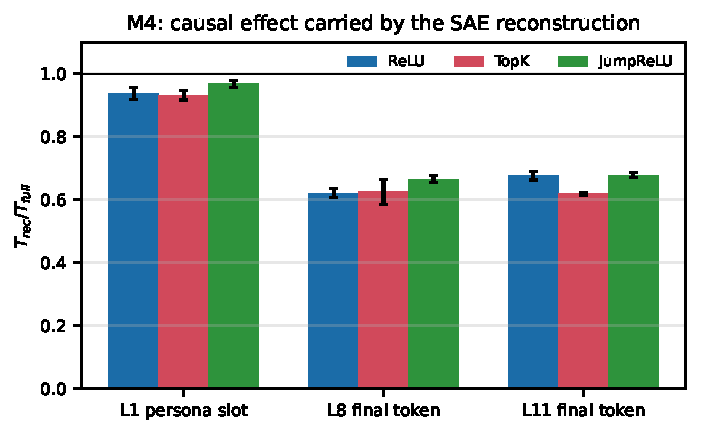
\includegraphics[width=0.62\linewidth]{fig_m4_preservation}
  \caption{M4 (\evlabel{validation}): share of the causal effect carried by the SAE-reconstructed activation
  difference ($T_{\text{rec}}/T_{\text{full}}$; mean$\pm$sd over 3 seeds; T2--T4).}
  \label{fig:m4}
\end{figure}

Whether fine-tuning changes this decomposition is tested in E3 (\S\ref{sec:e3}).

\pending{Minimum detectable effect statement (Review \#8 critique 3); M5 held-out confirmation.}

\section{Fine-tuning Experiments}\label{sec:finetune}

All fine-tuning starts from a trained SAE and runs 500 Adam steps (learning rate $10^{-5}$) with the sparsity
controller continued from the base coefficient; ReLU and JumpReLU must stay within $\pm$5\,\% of their base L0.
Truth is measured with probes fitted on original activations of GoT training groups B, which no training objective
sees.

\paragraph{A circular objective, found and corrected.} A truth-aware objective that distilled a linear probe's logits
appeared to remove most of the truth gap. An audit found that the evaluation probe was the training teacher (same
rows, labels and weights), so the result was circular. In a corrected design (teacher fitted on groups A, probes on B,
random-teacher control) the truth-aware objective is worse than plain reconstruction fine-tuning on every seed
(TopK B-MLP gap 0.189 vs 0.107; random teacher 0.165).

\paragraph{Method A and output-KL at layer 6.} Table~\ref{tab:ft6} reports Method A (GoT reconstruction with OWT
replay) and the output-KL variant. Method A cuts GoT reconstruction error by 72--82\,\% and lowers the independent MLP
truth gap on 18 of 18 paired comparisons against both the base and an OWT-only control, but never by more than 2 sd,
the pre-registered criterion (\evlabel{preliminary}). Adding output KL lowers OWT spliced KL (0.115$\to$0.102) and GoT
statement KL (0.110$\to$0.038) for TopK, meeting its behavioural criterion without changing the truth gap; for ReLU and
JumpReLU the KL term pushes L0 5--11\,\% above the base, so their gains are not creditable. A KL-weight ablation found
no truth trade-off to optimise (\evlabel{inconclusive}).

% generated by scripts/shared/build_paper_artifacts.py from results/geometry_of_truth/method_a_layer6/summary.csv, results/geometry_of_truth/e2e_inspired_layer6/summary.csv
\begin{table}[t]
\centering
\small
\caption{Layer-6 fine-tuning (VALIDATION; mean over 3 seeds). Method A lowered the B-MLP gap on 18/18 paired comparisons but never by more than 2 sd (pre-registered criterion not met). Output-KL rows for ReLU and JumpReLU fail the $\pm$5\% L0 guard and are not creditable. Source: \texttt{results/\allowbreak{}geometry\_of\_truth/\allowbreak{}method\_a\_layer6/\allowbreak{}summary.csv}; \texttt{results/\allowbreak{}geometry\_of\_truth/\allowbreak{}e2e\_inspired\_layer6/\allowbreak{}summary.csv}.}
\label{tab:ft6}
\begin{adjustbox}{max width=\linewidth}
\begin{tabular}{llccccc}
\toprule
SAE & Variant & GoT B-MLP gap $\downarrow$ & GoT rel. error $\downarrow$ & OWT EV $\uparrow$ & OWT $\Delta$CE $\downarrow$ & OWT L0 \\
\midrule
ReLU & Base & 0.321$\pm$0.022 & 0.059 & 0.828 & 0.177 & 134 \\
 & OWT-only control & 0.319$\pm$0.022 & 0.058 & 0.829 & 0.175 & 134 \\
 & Method A & 0.245$\pm$0.053 & 0.017 & 0.828 & 0.175 & 134 \\
 & Output-KL (B) & 0.280$\pm$0.020 & 0.024 & 0.830 & 0.145 & 141 \\
\midrule
TopK & Base & 0.203$\pm$0.030 & 0.034 & 0.853 & 0.104 & 128 \\
 & OWT-only control & 0.206$\pm$0.035 & 0.033 & 0.855 & 0.102 & 128 \\
 & Method A & 0.107$\pm$0.020 & 0.006 & 0.854 & 0.102 & 128 \\
 & Output-KL (B) & 0.114$\pm$0.022 & 0.009 & 0.852 & 0.091 & 128 \\
\midrule
JumpReLU & Base & 0.292$\pm$0.026 & 0.052 & 0.862 & 0.092 & 131 \\
 & OWT-only control & 0.287$\pm$0.027 & 0.052 & 0.864 & 0.091 & 131 \\
 & Method A & 0.238$\pm$0.056 & 0.015 & 0.863 & 0.091 & 131 \\
 & Output-KL (B) & 0.281$\pm$0.046 & 0.022 & 0.865 & 0.076 & 140 \\
\bottomrule
\end{tabular}
\end{adjustbox}
\end{table}


\subsection{Multi-layer improvement experiment (IMP-L)}\label{sec:impl}
\pending{Layers 3, 8 and 9; base vs OWT-only control vs Method A vs output-KL; 3 architectures $\times$ 3 seeds;
95\,\% $t$-intervals over seeds; L0 guards. Pre-registered in
\texttt{results/geometry\_of\_truth/multilayer\_finetune/preregistration.json}. Table generated from
\texttt{improvement\_table.csv} once the experiment has run.}

\subsection{Causal preservation after fine-tuning (E3)}
\pending{M4 decomposition at the layer-8 final token for the IMP-L layer-8 SAEs.}

\section{Statistical Analysis}\label{sec:stats}

\begin{itemize}
  \item \textbf{Pre-registration.} Every experiment from M0 onwards wrote its hypotheses, criteria and script hashes to
        \texttt{preregistration.json} before running; scripts refuse to overwrite outputs.
  \item \textbf{Within-layer inference (M0).} Fixed-effects regressions with Freedman--Lane permutation within layer
        (5000 permutations), bootstrap CIs (2000) and Holm correction over four primary pairs.
  \item \textbf{Information (M2).} Statement-grouped bootstrap (paired over the same rows), one-sided tests against
        noise and PCA references, Benjamini--Hochberg correction across SAEs per task; a 0.02 AUROC tolerance defines
        ``preserved''.
  \item \textbf{Causal (M3/M4).} Holm-corrected tests over 65 cells; 200 matched-norm random vectors per cell; synonym
        and neutral controls; for features, 200 random feature sets matched on activation frequency and $|\Delta z|$.
  \item \textbf{Seeds.} Three training seeds share the same training data, so seed spread understates uncertainty;
        comparisons that share seeds are paired. The fine-tuning criterion ``consistent'' requires the improvement on
        all three seeds and a mean paired difference larger than twice its standard deviation.
  \item \textbf{Splits.} Fitting and selection use training data; validation results are reported as
        \evlabel{validation}. Only the reconstruction table is \evlabel{test}.
\end{itemize}

\pending{M5: one pre-registered held-out pass (RepE-LM test, OWT test; GoT test labelled previously exposed),
hierarchical bootstrap over statements and seeds, Holm within confirmatory families.}

\section{Discussion}\label{sec:discussion}

\paragraph{Reconstruction is a proxy for behaviour, not for information.} Within a layer, an SAE with lower
reconstruction error damages the model's predictions less, but it does not keep more truth information. Reconstruction
metrics average over all directions weighted by their variance; the information that distinguishes true from false
statements, or honest from dishonest instructions, lies in small differences between nearly identical activations.

\paragraph{Why the causal effect leaks.} M4 makes this concrete. An SAE can reconstruct the honest and the dishonest
activation well individually and still reconstruct their difference poorly, because the two reconstruction errors do
not cancel. At mid and late sites about a third of the effect is outside the reconstructed difference, and for TopK
and JumpReLU part of it exists only when reconstruction and error act together through GPT-2's nonlinear downstream
computation.

\paragraph{What fine-tuning changes, and what it does not.} The fine-tuning experiments separate three things
that are often reported as one. (i) \emph{Task reconstruction} improves reliably: reconstruction error on truth
statements falls by 61--85\,\% in every cell. (ii) \emph{Frozen-probe preservation} improves in direction
everywhere and meets the pre-registered criterion in 4 of 9 cells, but a re-trained reader recovers no more truth
information from the fine-tuned reconstruction than from the original one (no cell changes consistently). Because M2
showed that frozen-probe gaps are dominated by the probe's sensitivity to off-distribution perturbations, the most
economical reading is that reconstruction fine-tuning moves the reconstruction back towards the region where the
original probe's decision boundary was fitted, rather than restoring information the SAE had discarded. (iii)
\emph{Behavioural preservation} improves with an output-KL term in all cells, and creditably in 5 of 9; it does not
transfer to truth preservation, which is unchanged or slightly worse. Improving one level of faithfulness therefore
does not improve the others, and a claim of ``more faithful SAEs'' must name the level.

\paragraph{Sparsity is part of the price.} For ReLU and JumpReLU at layers 8 and 9 the output-KL gain comes with a
5--8\,\% rise in L0 that the continued sparsity controller does not correct. Since lower reconstruction error and
lower KL are both easier at higher L0, behavioural gains reported without a sparsity guard would overstate the
benefit; TopK, whose L0 is fixed, is the only architecture where the gain is creditable at every layer.

\paragraph{The negative result is the main finding.} The SAEs studied here reconstruct well by conventional measures,
yet they lose task information that PCA at equal error keeps, and at mid and late layers their reconstruction carries
only part of a causal effect that GPT-2 demonstrably carries there. Short fine-tuning improves what it optimises
(task reconstruction, output agreement) and nothing we could verify beyond that. Whether fine-tuning also improves
\emph{causal} preservation is the open question addressed by E3. All of these are \evlabel{validation} findings.

\pending{Revise after E1--E3 and M5; in particular, whether the conclusions hold for an externally trained SAE
(E2) and at task-level matched sparsity (E1).}

\section{Limitations and Threats to Validity}\label{sec:limits}

\begin{itemize}
  \item \textbf{Small, data-limited SAEs.} 3072 latents (4$\times$), trained on 101{,}600 document-start tokens for
        about 38 passes, not converged (validation-based checkpoint selection always chose the final step). The public
        \texttt{gpt2-small-res-jb} SAE used 300M tokens and 24{,}576 latents. Conclusions may not transfer.
  \item \textbf{One operating point.} L0 = 128 and width 3072 only.
  \item \textbf{Surrogate JumpReLU.} Not the published estimator; up to 85\,\% dead latents at layer 0.
  \item \textbf{Task-level sparsity mismatch.} Matching is on OWT; task prompts activate very different numbers of
        latents per architecture.
  \item \textbf{Weak behavioural signal.} The persona effect is 0.02--0.04 nats; the persona-meaning gate passed
        narrowly (0.701).
  \item \textbf{Seeds share data.} Seed spread understates uncertainty.
  \item \textbf{Test exposure.} The GoT test split was scored in earlier frozen-probe evaluations; the original RepE
        test split was touched in a smoke run and is retired with the confounded task.
  \item \textbf{Single model.} No SAE results on Gemma-2-2B \citep{gemmateam2024gemma2}; Gemma Scope weights were
        not available on our machine.
\end{itemize}

\section{Conclusion and Future Work}\label{sec:conclusion}

Across all layers of GPT-2 Small, three SAE architectures reconstruct activations well by conventional measures, but
reconstruction quality predicts behavioural damage rather than information preservation, frozen-probe ``truth loss''
is largely perturbation sensitivity, SAEs never beat PCA at equal error on task information, and at mid and late
layers the SAE reconstruction carries only about two-thirds of a confirmed causal effect. Future work: larger and
longer-trained SAEs, the published JumpReLU estimator, task-level sparsity matching, and the same audit on Gemma-2-2B
with Gemma Scope SAEs.

\pending{Final conclusions after M5.}


\bibliographystyle{plainnat}
\bibliography{references}

\appendix
\section{Project History and Corrections}\label{app:history}

\begin{itemize}
  \item Layers were first trained with mixed optimiser procedures; all 108 SAEs were retrained with one uninterrupted
        15k-step protocol (explained variance changed by at most 0.006; rankings unchanged).
  \item An architecture summary averaged unmatched runs; it was replaced by a $\pm$10\,\% L0 matching rule.
  \item Earlier ``SAE steering'' never placed an SAE in the forward pass; it was reclassified.
  \item The truth-aware fine-tuning objective was circular (\S\ref{sec:finetune}).
  \item The original RepE persona prompts were length-confounded; RepE-LM replaces them.
  \item Correlations pooled across layers were replaced by within-layer analyses (M0).
  \item Frozen-probe failures were re-analysed with noise and PCA references (M2).
\end{itemize}
Historical results (original RepE probes and steering, the layer-6 causal test with 200 controls, R1 honesty
fine-tuning, R2 feature clamps, Gemma steering, Feature 974) are kept in the repository with their status labels and
are not used as evidence here.

\section{Test-split Exposure}\label{app:exposure}
OWT test: used once, for the reconstruction table. GoT test: scored for all 108 SAEs with frozen probes and twice for
historical layer-6 fine-tunes. RepE-LM test: never built or accessed. M0--M4 used no test rows.

\section{Reproducibility}\label{app:repro}
Code, configurations, pre-registrations and result files: repository \texttt{Fall2026group4/fall-2026-group4}, branch
\texttt{sae-research}. Software: Python 3.14, PyTorch 2.14.1, TransformerLens 3.9.0 \citep{transformerlens2022},
transformers 5.21.0, SAELens 6.54.12. Hardware: one NVIDIA A10G (23 GB). Tables and figures in this paper are generated
by \texttt{scripts/shared/build\_paper\_artifacts.py} from the committed result files. SAE checkpoints (about 9 GB)
are listed with SHA-256 hashes in \texttt{docs/checkpoint\_registry.csv}.

\pending{Command list per experiment; pipeline diagram (Review \#8 F8: \texttt{.drawio} source and \texttt{.svg}).}


\end{document}
